% Created 2023-03-19 Sun 10:32
% Intended LaTeX compiler: pdflatex
\documentclass[11pt]{article}
\usepackage[utf8]{inputenc}
\usepackage[T1]{fontenc}
\usepackage{graphicx}
\usepackage{longtable}
\usepackage{wrapfig}
\usepackage{rotating}
\usepackage[normalem]{ulem}
\usepackage{amsmath}
\usepackage{amssymb}
\usepackage{capt-of}
\usepackage{hyperref}
\author{Yusheng Zhao}
\date{\today}
\title{Problem 6}
\hypersetup{
 pdfauthor={Yusheng Zhao},
 pdftitle={Problem 6},
 pdfkeywords={},
 pdfsubject={},
 pdfcreator={Emacs 28.2 (Org mode 9.6)}, 
 pdflang={English}}
\begin{document}

\maketitle
\tableofcontents


\section{Problem 1}
\label{sec:orgb5dcc9b}
\begin{itemize}
\item Phase velocity is \(v_{p} = \frac{\omega}{k} = \sqrt{\frac{4C}{Mk^{2}}}|\sin(\frac{1}{2}ka)|\)
\item Group velocity is \(v_{g} = \frac{\partial \omega}{\partial k} = \pm \sqrt{\frac{4C}{M}}\frac{a}{2} \cos(\frac{1}{2}ka)\)

\item In the following plot, I made \(a=1\) and \(4C/M=1\)
\begin{verbatim}
using Plots
vp(k) = abs(sin(k/2))/abs(k)
vg(k) = k >= 0 ? cos(k/2)/2 : - cos(k/2)/2
k = -π:0.001:π
vps = vp.(k)
vgs = vg.(k)
plot(k,vps;title="k vs. Phase Velocity",label="Velocity")
xlabel!("k 1/angstrom")
ylabel!("velocity anstrom/sec")
savefig("phase.png")
plot(k,vgs;title="k vs. Group Velocity",label="Velocity")
xlabel!("k 1/angstrom")
ylabel!("velocity anstrom/sec")
savefig("group.png")
\end{verbatim}
\end{itemize}

\begin{center}
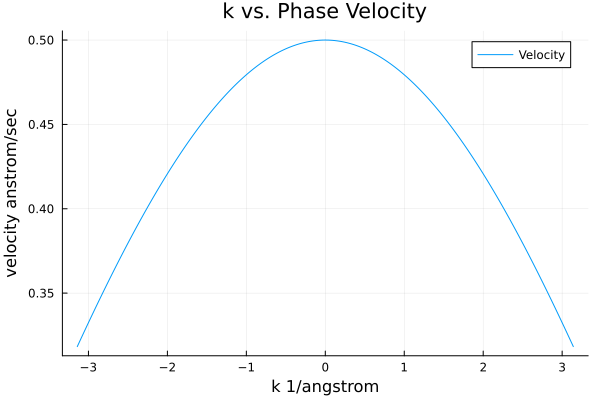
\includegraphics[width=.9\linewidth]{./phase.png}
\end{center}
\begin{center}
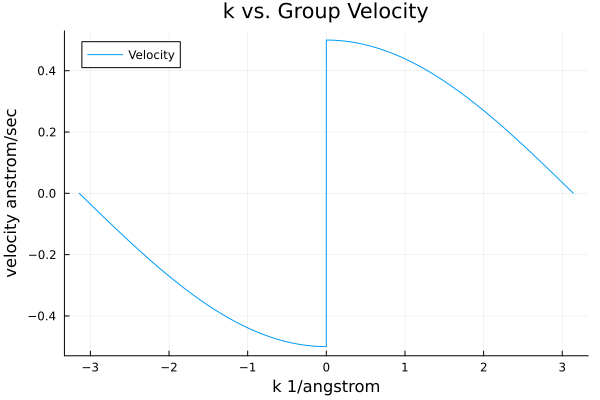
\includegraphics[width=.9\linewidth]{./group.png}
\end{center}

\section{Problem 2}
\label{sec:orgbacda00}
\begin{itemize}
\item At small \(k\) we assume linear relation between phonon momentum and \(\omega\).
Therefore \(v_{s} = v_{p}|_{k \ll 1} = \frac{\omega}{k} =
  \sqrt{\frac{4C}{Mk^{2}}}|\sin(\frac{1}{2}ka)| \approx
  \sqrt{\frac{C}{M}}a\).
\item Since the chain density is \(\rho = M/a\), for \(v_{s} \equiv \frac{1}{\sqrt{\beta \rho}}\), \(\beta = \frac{1}{aC}\)
\end{itemize}
\end{document}